% !TEX root = slides.tex

\section{Case Study}

\againframe{overview}

\begin{frame}
    \frametitle{Simulation}
    
    \begin{itemize}
        \item Model predictive control
        \begin{itemize}
            \item Formulated using Pyomo and OMLT
            \item Solved using CBC 
        \end{itemize}
        \item Manual control
        \begin{itemize}
            \item 16 hours photoperiod starting at 4 o'clock
            \item $12.9 \, \mathrm{mol} \, \mathrm{m}^{-2} \, \mathrm{d}^{-1}$ optimal accumulated irradiance
            \item $3.8 \, \mathrm{mol} \, \mathrm{m}^{-2} \, \mathrm{d}^{-1}$ average accumulated natural irradiance 
        \end{itemize}
        \item Forecasts of the uncertain inputs
        \begin{itemize}
            \item Solar forecasts from external service
            \item Persistence forecast of temperature and humidity
            \item Seasonal persistence forecast of carbon dioxide concentration 
        \end{itemize}
        \item Time from the 10th to 15th Decemer 2022
    \end{itemize}
\end{frame}

\begin{frame}
    \frametitle{Results}
    \begin{figure}
        \centering
        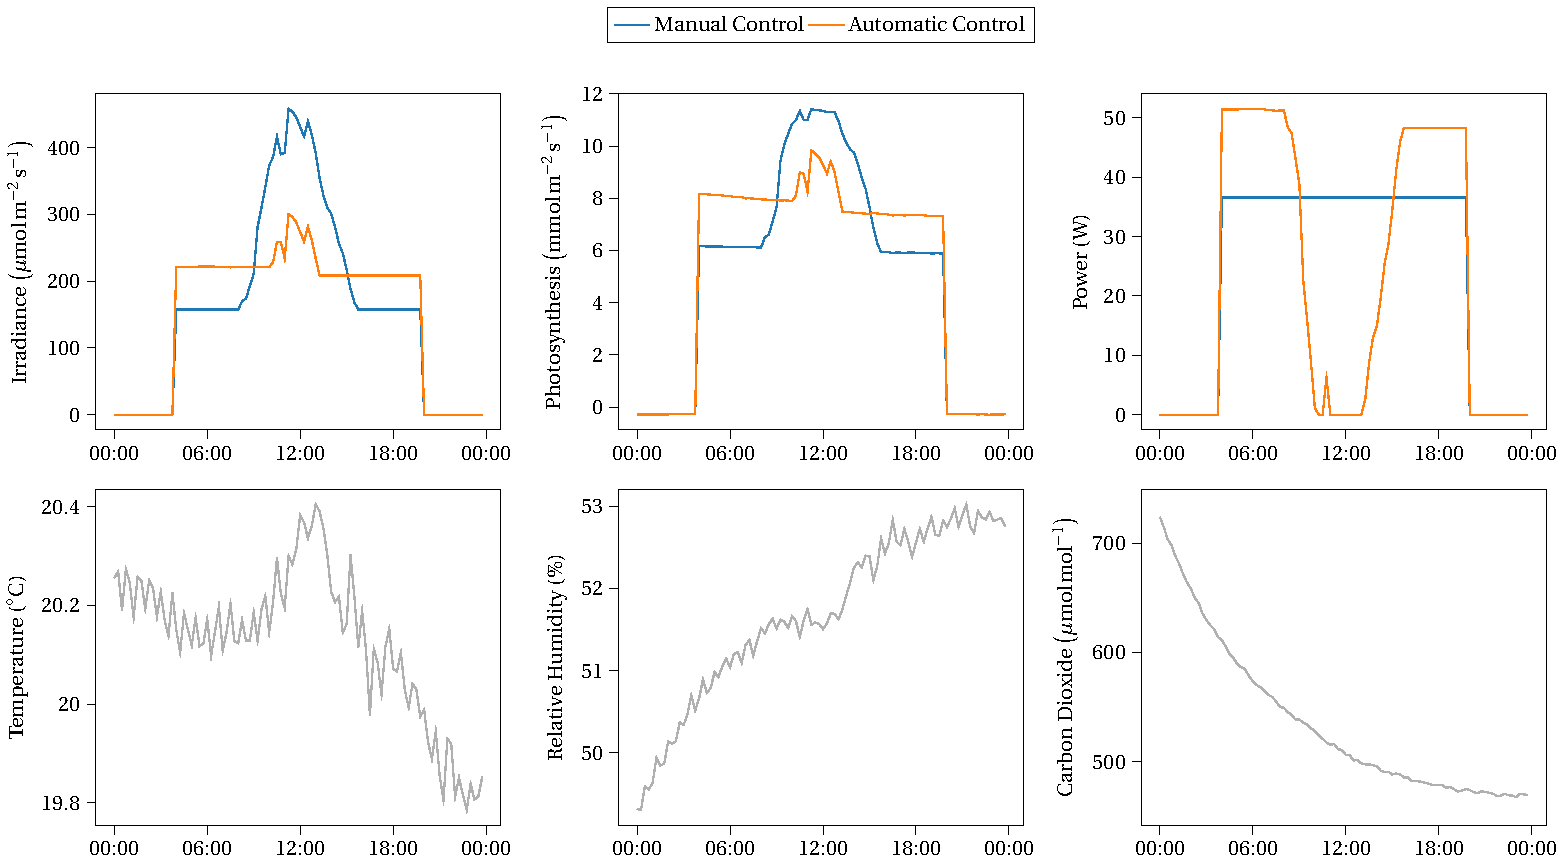
\includegraphics[scale=0.3]{figures/casestudy.pdf}
        \caption{Results of the simulation case study for 10th December 2022.}
    \end{figure}
\end{frame}

\begin{frame}
    \frametitle{Results}
    \begin{table}
        \centering
        \resizebox{10cm}{!}{
            \begin{tabular}{lrrrrr}
            \toprule
            & 10.12.2022 & 11.12.2022 & 12.12.2022 & 13.12.2022 & 14.12.2022 \\
            \midrule
            manual & 13.59 & 11.71 & 10.38 & 14.86 & 14.6 \\
            automatic & 12.9 & 11.79 & 10.45 & 12.95 & 12.9 \\
            \bottomrule
            \end{tabular}
        }
        \caption{Accumulated irradiances $\left(\mathrm{mol} \, \mathrm{m}^{-2} \, \mathrm{d}^{-1}\right)$}
    \end{table}
\end{frame}

\begin{frame}
    \frametitle{Results}
    \begin{table}
        \centering
        \resizebox{10cm}{!}{
            \begin{tabular}{lrrrrr}
            \toprule
            & 10.12.2022 & 11.12.2022 & 12.12.2022 & 13.12.2022 & 14.12.2022 \\
            \midrule
            manual & 742.81 & 659.95 & 658.19 & 854.64 & 784.81 \\
            automatic & 832.15 & 674.58 & 670.92 & 1065.63 & 933.17 \\
            \bottomrule
            \end{tabular}
        }
        \caption{Ratios of accumulated photosynthetic rates per power unit $\left(\mathrm{mmol} \, \mathrm{m}^{-2} \, \mathrm{d}^{-1} \; \slash \; \mathrm{kWh}\right)$}
    \end{table}
\end{frame}